\documentclass[12pt, letterpaper]{article}
\usepackage[utf8]{inputenc}
\usepackage[czech]{babel}
\usepackage[normalem]{ulem}
\usepackage{amsmath}
\usepackage{indentfirst}
\usepackage{listings}
\usepackage{caption}
\usepackage{float}
\usepackage{graphicx}
\usepackage{hyperref}
\usepackage{textcomp}
\usepackage{array}
%%%
%%%
\begin{document}
%%%
%%% TITLE PAGE
%%%
\begin{titlepage}
\centerline{
\includegraphics[width=10cm]{img/logo}}
\begin{center}
\vspace{30px}
{\huge
\textbf{Databázové systémy a metody zprac.inf.2}\\
\vspace{1cm}
}
{\Large
\textbf{KIV/DBM2}\\
\vspace{1cm}
}
{\large
\textbf{Porovnání úspěšnosti dle formy studia}\\
\vspace{1cm}
}
\vspace{1cm}
{\large
Pavel Třeštík\\
}
{\normalsize
A23N0001P
}
\end{center}
\vspace{\fill}
\hfill
\begin{minipage}[t]{7cm}
\flushright
\today
\end{minipage}
\end{titlepage}
%%%
%%% TEXT START - Uvod
%%%
\section{Téma a motivace}
Vybraným tématem je \uv{porovnání úspěšnosti dle formy studia}. Hlavním cílem je zjistit úspěšnost každé formy studia
(prezenční, kombinované a distanční) a porovnat tyto úspěšnosti. Výsledkem tohoto porovnání by mělo být přibližně
stejné procento úspěšnosti.

Termín \uv{úspěšnost} byl již použit a nejjednodušší statistickou metrikou pro úspěšnost by byl jednoduše podíl
absolventů ku všem studentům. Tato práce by ovšem neměla moc velký smysl, kdyby pro její dokončení stačilo 
udělat 3 podíly. Úspěšnost je zde pro nás tedy něco převážně neznámého a cílem práce je vybrat vhodné příznaky, které
nám úspěšnost vytvoří. Tato úspěšnost bude založena převážně na známkách. Známky jsou prakticky určeny k tomu, aby
ohodnocovaly studentovu úspěšnost. Čistě známka ovšem může být zkreslující údaj sám o sobě, protože předměty mohou
mít různé kreditové ohodnocení (tedy váhu), statut (A/B/C) a další. Také může hrát roli např. na kolikátý pokus
student známku dostal nebo jestli předmět opakuje.

Počítání úspěšnosti tímto způsobem by mohlo být možné analyticky či některým modelem strojového učení. V případě, že by
úspěšnost závisela na pouze malém počtu vlastností, jejichž důležitost je jasně daná, tak by bylo možné úspěšnost 
pouze vypočítat a výsledkem práce by mohl být pouze SQL skript. Při větším počtu vlastností nebo problémy s určením
jejich vah, bude nutné použít jiný přístup, kterým by nejspíše byl nějaký regresní algoritmus strojového učení. Důvodem
proč by se mohlo jednat o regresní úlohu je, že práce má vyjádřit úspěšnost pro danou formu studia. Otázkou ale je,
jak bude tato úspěšnost počítána.
%%%
%%% Analyza
%%%
\section{Analýza}
Pro realizaci práce je poskytnuta \textbf{demo} databáze (Oracle), ve které jsou anonymizovaná data STAGu. Tato
databáze se skládá z několika stovek tabulek. K databázi je také poskytnut diagram, který reprezentuje jádro 
databáze a vazby mezi nejdůležitějšími entitami. Z tohoto diagramu by mělo být dohledatelné, kde se nachází 
nejrelevantnější informace.

V sekci téma a motivace je stručně popsáno, že tato práce má za cíl hodnotit úspěšnost dle formy studia. Sekce také 
popisuje, že \uv{úspěšnost} je zde chápána jako sofistikovanější veličina, než jednoduchý podíl úspěšných studentů ku 
všem. Sekce také uvádí příklady možných metrik pro určení úspěšnosti (např. kolikátý pokus splnění, počet kreditů za 
známku, atd.). Hlavní metrikou pro určování úspěšnosti jsou známky a údaje k známce relevantní. Proto dává smysl 
začít průzkum databáze od tabulky \textbf{ZNAMKY}, která je součástí jádra databáze.

V úvodní sekci jsou také zmíněny dva přístupy ke zpracování získaných dat. První způsob by byl realizován pouze
výpočtem úspěšnosti pro každou formu studia. Tento výpočet by byl obsah SQL skriptu, který by sloužil jako výstup této 
práce. Druhý způsob je aplikování strojového učení a vytvoření modelu, který bude predikovat úspěšnosti pro každou 
formu studia. 

Ačkoliv jsou oba přístupy validní, tak vymyslet vzoreček pro počítání úspěšnosti se nejeví jako jednoduchá úloha pro
člověka. Jedním faktorem je počet metrik, které budou úspěšnost určovat a druhým faktorem je důležitost každé metriky,
kterou člověk dokáže sice odhadnout, ale pouze těžko ji dokáže vyčíslit přesným reálným číslem v relevanci k ostatním 
metrikám. Z tohoto důvodu bude pro realizaci práce použito strojové učení.

Protože práce bude vytvářet model strojového učení, tak se nabízí možnost vybrat co největší množství sloupců z databáze
a použitím nástroje \textbf{weka} použít funkci \texttt{Select attributes}, která by měla ohodnotit vybrané sloupce 
podle důležitosti k modelu.

Stále je ale nutné vybrat vhodné sloupce manuálně, protože některé metriky jsou prakticky zbytečné a nebo by 
znehodnotily používaný model. Příklady zbytečných údajů jsou například datumy vložení či updatování záznamu, vlastník
záznamu, atp. Příklady znehodnocujících sloupců jsou například ID, osobní čísla nebo jména. Ačkoliv se vliv na model
může lišit podle toho a jakou metriku se jedná, tak jedním z hlavních problémů použití těchto sloupců je ztráta 
generalizace, protože pomocí těchto sloupců je možné konkrétně identifikovat jeden konkrétní záznam. Další možnou
nevýhodou by byl čas běhu, protože čím více metrik model bude mít, tím pomalejší bude trénování modelu a případně
predikce celé množiny.

Nakonec analýzy je třeba vybrat vhodný model. Modelů je celá řada a první dělení je mezi model s učitelem a nebo bez
učitele. Rozdíl mezi těmito dvěma modely je, že pro model s učitelem potřebujeme mít učící množinu se známými výsledky.
Modely s učitelem se dále dělí na regresní a klasifikační. Regresní model predikuje reálné číslo. Klasifikační model
zařazuje záznam (objekt na vstupu) do jedné třídy z konečné množiny tříd. Následkem je, že pro použití modelu s 
učitelem, je potřeba najít způsob vytvoření trénovací množiny, která bude mít přiřazené správně hodnoty či třídu.
Naopak učení bez učitele sice nepotřebuje správné výsledky v trénovací množině, ale výsledkem budou nějaké shluky prvků,
které bude nejspíš potřeba manuálně nějak označit. Učení bez učitele je tedy nazýváno shlukování a je dostupných 
několik shlukovacích algoritmů. 

Výběr modelu proto bude záviset na vybraných datech, protože teoreticky je možné úlohu realizovat kterýmkoliv typem 
modelu. V případě regresního modelu by výsledné číslo znamenalo míru úspěšnosti ve formě studia. V případě klasifikace 
by vybraná třída značila nejpravděpodobnější úspěšnost. A v případě shlukování vzniknou shluky podobných instancí, 
které lze prakticky chápat jako třídy u klasifikace.
%%%
%%% Realizace
%%%
\section{Realizace}
Realizace úlohy má 2 hlavní části. První částí je seznámit se s poskytnutou \textbf{demo} databází a vybrat vhodné 
informace pro dosažení výsledků práce. V druhé části se data, která byla v první části vybrána, zpracují a použijí
se k vytvoření modelu, který dá výsledné úspěšnosti. Model se poté aplikuje na zvolená data a výsledky se mohou 
porovnat například se zmíněnou statickou úspěšností (podílem úspěšných studentů ku všem).
%%%
%%%
\subsection{Výběr a příprava dat}
První krok pro výběr dat bylo se seznámit s databází a alespoň hlavní strukturou, která se vztahuje k tématu práce.
Databáze je provozována na \texttt{Oracle} a k připojení byl použit program \texttt{DBeaver (CE)}. K připojení nám
byly poskytnuty údaje pro uživatele se schématem \textbf{INSTALL}, ale data pro práci jsou umístěna ve schématu
\textbf{INSTALL2}, ke kterému má tento uživatel přístup.

Výběr vhodných dat začal manuální inspekcí sloupců tabulky známky a hledáním relevantních tabulek. Hledání relevantních
tabulek bylo realizováno zkoumáním diagramu jádra databáze a použitím SQL dotazu pro získání všech tabulek s vazbou
na zvolenou tabulku. Inspekce sloupců byla prováděna pomocí jména a popisků. Tato fáze ale byla pouze průzkum pro 
zjištění hrubého odhadu sloupců a tabulek, které budou použity pro získání potřebných dat.

Dle analýzy stačilo vybrat pouze tabulky a \uv{vyhodit} nevhodné sloupce. Inspekcí ovšem bylo zjištěno, že toto nebude
vhodný přístup. Některé tabulky mají desítky sloupců a proto bylo usouzeno, že je lepší vytipovat a vybrat sloupce 
manuálně. Manuálním výběrem samozřejmě můžeme přijít o část relevantních sloupců, ale vybrané sloupce by měly sloužit
jako důležitější metriky, než kterýkoliv náhodný sloupec. Ztráta málo relevantních sloupců by neměla mít příliš velký
dopad na výsledný model.

Výsledná data tvořící dataset je 13 sloupců z 4 tabulek. Jedná se o tabulky \textbf{ZNAMKY}, 
\textbf{STUDIJNI\_PROGRAMY}, \textbf{STUDENTI\_V\_ROCE} a \textbf{STUDENTI}. Pro správný výběr jsou použity dodatečné 
tabulky, které slouží k filtrování vybraných záznamů. Většina vybraných sloupců by měla být 
sebe vysvětlující, ovšem je pár sloupců, jejich výběr je vhodné odůvodnit.
%
\begin{itemize}
    \item \textbf{STUDIJNI\_PROGRAMY.FORMA} na první pohled se může zdát, jako údaj, který model znehodnotí, protože 
        přesně udává formu studia. To je ovšem správně, protože účel modelu je predikování úspěšnosti dle formy 
        studia, tedy forma studia je nám známá podmínka.
    \item \textbf{STUDENTI\_V\_ROCE.ROK\_PLATNOSTI} jedná se o rok studia. Je to potenciálně údaj, který může narušovat
        generalizaci, jako např. přesný datum vložení. Záměrem proč je rok v modelu je zjistit, jestli úspěšnost závisí
        na roku studia. Rok také nemusí být použit individuálně, ale mohou být vytvořeny intervaly po např. 5ti letech.
\end{itemize}

Vybraná data jsou relevantní ke známce a ne ke studentům. Úspěšnost je zde tedy zaměřena spíše na známky, ale některé 
data pochází ze studentů. Příkladem je boolean sloupec \textbf{STUDENTI.NOVE\_PRIJATY}. Naopak není použit třeba 
průměr studentů. Protože data pochází primárně ze známek, znamená to, že pro každého studenta mohou existovat desítky
záznamů, ze kterých je tvořený model.
%%%
\subsubsection{Problémy}
Při výběru vhodných tabulek a sloupců byly řešeny problémy, které ovlivnily výběr dat či dokonce výběr modelu. Celkově
byla data vybírána s ohledem na to, který model by bylo vhodné použít.

S výběrem samotných dat byl občas problém dohledat vhodnou entitu a nebo pochopit účel sloupce pouze na základě jména
a velmi stručného popisku. Příkladem je, jak získat úspěšné absolventy. V tabulce \textbf{STUDENTI} je sloupec 
\textbf{Absolvent} s popisem \uv{\texttt{Absolvent}}, datovým typem \texttt{VARCHAR2(1)} a hodnotami \texttt{A}, 
\texttt{B}. Díky datovému typu a hodnotám tedy tušíme, že se jedná o boolean, ale znamená to, že studen úspěšně 
absolvoval studium? Nebo to znamená, že student teprve bude studium absolvovat?

Konkrétně k problému s vybráním absolventů, tak v databázi je také tabulka \textbf{ABN\_ABSOLVENTI}, která je na 
studenty vázána osobním číslem. Práce tedy předpokládá, že v této tabulce jsou vedeni absolventi. I tak zde je ale 
problém a tím je, že při \texttt{INNER JOIN} tabulek \textbf{ABN\_ABSOLVENTI} a \textbf{STUDENTI} nám vznikají dvojice,
kdy \textbf{STUDENTI.Absolvent} je \textbf{N}, ale záznam v \textbf{ABN\_ABSOLVENTI} existuje, tedy student je 
absolvent. Je tedy \textbf{Absolvent} relevantní údaj? Čemu věřit? Tato práce věří \textbf{ABN\_ABSOLVENTI}, takže
pokud student má záznam v této tabulce, tak je považován za úspěšného absolventa.
%%%
\subsubsection{Výsledek}
Práce je odevzdána s SQL skriptem \texttt{full\_data\_preparation.sql}. Spuštění tohoto skriptu nad \textbf{demo} databází vybere data, která tato 
práce dále používá k vytvoření modelu a následně získání výsledku. Vybraná data záměrně umožňují duplikáty záznamů, 
protože pokud by byl použit model jako neuronová síť, tak i když jsou záznamy duplicitní, tak mají hodnotu, protože
tím mají větší váhu pro své hodnoty. V době odevzdání práce má skript následující metriky:
%
\begin{table}[H]
    \begin{center}
        \begin{tabular}{ | m{0.5\textwidth} | m{0.5\textwidth} | }
            \hline
            Čas běhu                     & $\sim$13s \\
            \hline
            Záznamů celkem               & 2722101 \\
            \hline
            Unikátních záznamů           & 461120 \\
            \hline
            Velikost                     & $\sim$111MB \\
            \hline
        \end{tabular}
        \caption{Metriky připravených dat}
        \label{table:data_metrics}
    \end{center}
\end{table}
%%%
%%%
\subsection{Výběr modelu}
Na základě analýzy máme tři možné typy modelů, které může práce využít. Výběr modelu byl značně ovlivněn inspekcí a 
přípravou dat.

Během přípravy dat byl čím dál více zjišťován omezující faktor výběru modelu a tím je určení hodnot, které by mohly
být použity k učení s učitelem. Před začátkem práce se předpokládalo použití regresního modelu. Vybíráním dat bylo
zjištěno, že není žádný vhodný způsob, jak získat hodnoty pro trénovací množinu. Kvůli tomu není možné použít 
regresní model, protože bez správných výsledků v trénovací množině nelze realizovat učení s učitelem.

Zde vznikl nápad použít shlukování na data. Shluky by pak mohly být použity k vytvoření hodnot, které by umožnily 
vytvoření regresního modelu. Hodnoty by mohly být získány např. výpočtem velikosti vektoru. Tento nápad byl ovšem
opuštěn, protože by vyžadoval vytvoření shlukového modelu, aby mohl být vytvořen regresní model a také výsledné hodnoty
by mohly být problémové. Bylo by třeba řešit problémy jako 2 vektory se stejnou velikostí patří do jiných shluků, což
by znamenalo, že se nemůže jednat o stejnou úspěšnost. Kvůli tomu je velikost vektoru nedostatečně deterministická
k určení úspěšnosti, protože např. vektor známek 4 bude mít stejnou velikost jako vektor známek 1, protože oba vektory 
jsou outlieři.

Regresní model byl tedy shledán jako nerealizovatelný a to i v kombinaci se shlukováním. Protože shlukování je něco jako
\uv{klasifikace bez učitele}, tak realizace práce přešla na klasifikační model. Zjištění třídy klasifikace pro tuto úlohu
je velmi prosté, protože stačí zkombinovat formu studia s úspěšností absolvování. Třídou tedy je zmíněný podíl
úspěšných absolventů ku všem studentům na dané formě studia. Takováto třída je jednoduché řešení, jak vytvořit model 
pro sofistikovanější predikci úspěšnosti založený na statistických datech. Práce tedy používá klasifikační model 
s 6ti třídami.
%%%
%%%
\subsection{Zpracování dat do modelu}
Nyní je vybrán typ modelu. Pro klasifikační model je řada implementací, mezi nejznámější patří: Logistická regrese, 
Naivní Bayes, SVM či neuronové sítě. 
\begin{itemize}
    \item Logistická regrese je vhodná pro binární použití, takže pro tuto práci nevyhovuje.
    \item Naivní Bayes je velice dobrý klasifikátor vzhledem k jeho jednoduchosti. Pro správnou funkci by vlastnosti modelu měly 
        být nezávislé, ale v této práci jsou naopak velmi závislé. Navzdory porušení této podmínky funguje Naivní Bayes stále 
        velmi dobře na řadu úloh a vzhledem k jeho rychlosti učení byl použit pro většinu zpracování.
    \item SVM jsou také velmi dobré klasifikátory, které navíc mohou využívat tzv. kernely k modelovaní velmi přesných 
        rozhodovacích hranic. Výhodou SVM je, že stačí relativně málo dat k naučení modelu. Práce původně měla 
        využívat SVM model k porovnání s naivním Bayesem, aby bylo možné ověřit spolehlivost Bayes klasifikátoru. 
        Doba trénování SVM je ale mnohem delší než Bayes klasifikátor a použití tohoto modelu bylo moc časově náročné 
        při realizaci práce.
    \item Neuronové sítě jsou asi nejznámější a nejsofistikovanější modely strojového učení. Jejich nevýhodou je 
        potřeba velkého objemu dat k naučení a dlouhá doba učení. Kvůli těmto nevýhodám práce neuronové sítě nepoužívá.
\end{itemize}

Pro vytvoření modelů byl použit nástroj \textbf{weka}, který byl učen na cvičení. Weka poskytuje implementace pro řadu
algoritmů, kterými jsou i vybraný \textbf{NaiveBayes} a implementace SVM známá jako \textbf{SOM}.

Vytvořením modelu a provedením experimentu je získána očekávaná úspěšnost dle modelu. Tuto úspěšnost porovnáme proti 
statistické a tím získáme zjistíme, jestli je úspěšnost závislá na vybraných datech - tj. známka, kredity za známku, 
počet pokusů, atd.

Při výběru dat je zmíněn \textbf{ROK\_PLATNOSTI} jako potenciálně důležitý údaj. Byly vytvořeny modely, kdy byly roky
použity individuálně, jako intervaly a dokonce kompletně vynechány. Tyto modely se mají minimální rozdíl ve výsledcích
a proto bylo usouzeno, že \textbf{ROK\_PLATNOSTI} není relevantní pro úspěšnost studentů nezávisle na formě studia.

Bylo vytvořeno několik dalších modelů testující relevantnost atributu tím, že byl atribut z modelu odstraněn. Některé 
atributy také měly minimální dopad na výsledky modelu a byly shledány irelevantní jako \textbf{ROK\_PLATNOSTI}.
%%%
%%% Vysledky
%%%
\section{Výsledky}
Práce měla porovnat úspěšnost dle formy studia. Důležité je zmínit, že výsledky nejsou poměr absolventů a studentů, 
ale poměr záznamů reprezentující známku a dodatečné informace k ní. Pro porovnání hlavních výsledků lze použít 
statistický podíl, proti výsledkům modelu.
\begin{table}[H]
    \begin{center}
        \begin{tabular}{ | c || c | c | }
            \hline
                        & Stat.     & N. Bayes    \\
            \hline \hline
            prezenční   & $\frac{335335}{2406529} = 13.93\%$    & $\frac{143168}{2406529} = 5.95\%$ \\
            \hline
            kombinované & $\frac{27727}{296209} = 9.36\%$       & $\frac{16371}{296209} = 5.53\%$   \\
            \hline
            distanční   & $\frac{2708}{19363} = 13.99\%$        & $\frac{1040}{19363} = 5.37\%$     \\
            \hline
        \end{tabular}
        \caption{Porovnání úspěšnosti modelu a statistiky}
        \label{table:main_result}
    \end{center}
\end{table}

Z tabulky \ref{table:main_result} vidíme, že výsledky modelu jsou značně horší, než reálné úspěšnosti. Důvodem nejspíš
je, že model velmi často zařazuje výsledky do opačné třídy. To naznačuje, že model je pravděpodobně nedostatečně 
obsáhlý proto, aby dokázal správně predikovat úspěšnost. Na obrázku \ref{fig:bayes_results} lze vidět výsledek klasifikace tímto modelem.
\begin{figure}[H]
    \centering
    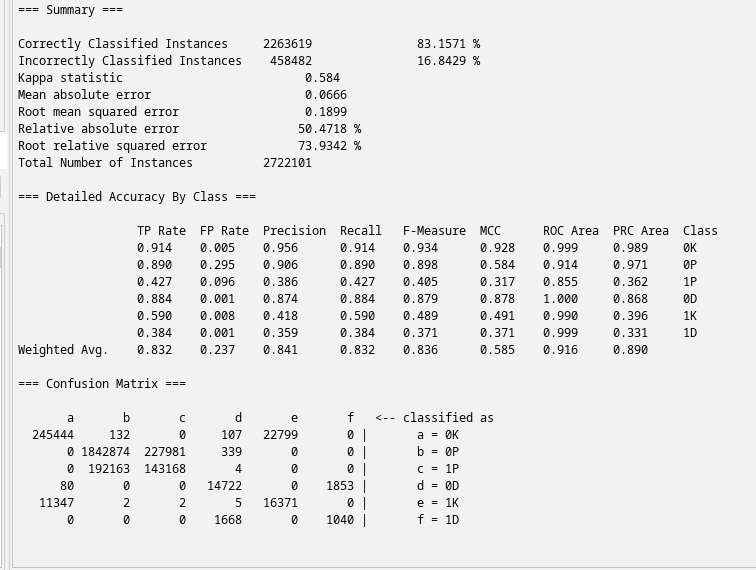
\includegraphics[width=\linewidth]{img/results_bayes.png}
    \caption{Výstup N. Bayes klasifikátoru}
    \label{fig:bayes_results}
\end{figure}
%%%
Dále se ukázalo že z vybraných 13ti atributů, jsou některé téměř irelevantní a proto mohly být z datasetu odstraněny s
minimálním dopadem na výsledky. Tabulka \ref{table:features} reprezentuje vybrané atributy. Odstraněné atributy jsou 
přeškrtnuty. Všechny odstraněné atributy jsou z tabulky \textbf{STUDENTI} a výsledky klasifikace bez těchto atributů
jsou v některých případech i lehce lepší, než s nimi.
\begin{table}[H]
    \begin{center}
        \begin{tabular}{ | c | c | }
            \hline
            Sloupec                       & Alias \\
            \hline \hline
            \sout{NOVE\_PRIJATY}                  & \sout{STD\_NOVE\_PRIJATY}      \\
            \hline
            \sout{STUPEN\_PRED\_VZDELANI}          & \sout{STD\_STUPEN\_PRED\_VZDELANI}      \\
            \hline
            \sout{POCET\_ZAPISOVYCH\_PROPUSTEK}    & \sout{STD\_POCET\_PROPUSTEK}      \\
            \hline
            FORMA                         & SP\_FORMA      \\
            \hline
            FAKULTA\_SP                    & SP\_FAKULTA\_PROGRAMU      \\
            \hline
            \sout{ROK\_PLATNOSTI}                 & \sout{SVR\_ROK}      \\
            \hline
            POC\_KRED                      & ZN\_KREDITY\_ZA\_PREDMET      \\
            \hline
            STATUT                        & ZN\_STATUT\_PREDMETU      \\
            \hline
            POKUS\_CISLO                   & ZN\_POKUS\_CISLO      \\
            \hline
            HODNIDNO\_ZKZP                 & ZN\_HODNOCENI      \\
            \hline
            TYP\_ZK                        & ZN\_TYP\_ZKOUSKY      \\
            \hline
            PRAC\_ZKR                      & ZN\_PRACOVISTE\_ZKRATKA      \\
            \hline
            ZAPOCET\_POKUS                 & ZN\_ZAPOCET\_POKUS      \\
            \hline
        \end{tabular}
        \caption{Použité vlastnosti}
        \label{table:features}
    \end{center}
\end{table}
% \begin{table}[H]
%     \begin{center}
%         \begin{tabular}{ | c | c | c | }
%             \hline
%             Tabulka             & Sloupec                       & Alias \\
%             \hline \hline
%             STUDENTI            & NOVE\_PRIJATY                  & STD\_NOVE\_PRIJATY      \\
%             \hline
%             STUDENTI            & STUPEN\_PRED\_VZDELANI          & STD\_STUPEN\_PRED\_VZDELANI      \\
%             \hline
%             STUDENTI            & POCET\_ZAPISOVYCH\_PROPUSTEK    & STD\_POCET\_PROPUSTEK      \\
%             \hline
%             STUDIJNI\_PROGRAMY   & FORMA                         & SP\_FORMA      \\
%             \hline
%             STUDIJNI\_PROGRAMY   & FAKULTA\_SP                    & SP\_FAKULTA\_PROGRAMU      \\
%             \hline
%             STUDENTI\_V\_ROCE     & ROK\_PLATNOSTI                 & SVR\_ROK      \\
%             \hline
%             ZNAMKY              & POC\_KRED                      & ZN\_KREDITY\_ZA\_PREDMET      \\
%             \hline
%             ZNAMKY              & STATUT                        & ZN\_STATUT\_PREDMETU      \\
%             \hline
%             ZNAMKY              & POKUS\_CISLO                   & ZN\_POKUS\_CISLO      \\
%             \hline
%             ZNAMKY              & HODNIDNO\_ZKZP                 & ZN\_HODNOCENI      \\
%             \hline
%             ZNAMKY              & TYP\_ZK                        & ZN\_TYP\_ZKOUSKY      \\
%             \hline
%             ZNAMKY              & PRAC\_ZKR                      & ZN\_PRACOVISTE\_ZKRATKA      \\
%             \hline
%             ZNAMKY              & ZAPOCET\_POKUS                 & ZN\_ZAPOCET\_POKUS      \\
%             \hline
%         \end{tabular}
%         \caption{Porovnání úspěšnosti modelů a statistiky}
%         \label{table:main_result}
%     \end{center}
% \end{table}
%%%
%%% Zaver
%%%
\section{Závěr}
Z výsledků porovnání vzniklého modelu ku statistickému podílu je vidět, že model je velmi nepřesný, až skoro 
nepoužitelný. Při inspekci použitých atributů bylo zjištěno, že některé atributy model téměř zhoršovaly. Je možné, že
úspěšnost modelu by dosáhla lepších čísel s větším počtem atributů. Ale také je možné, že zkrátka nelze lépe
předpovídat úspěšnost formy studia se známkami jako hlavní zdroj informací.
%%%
%%%
\end{document}
